\begin{figure}[H]
	\centering
	% 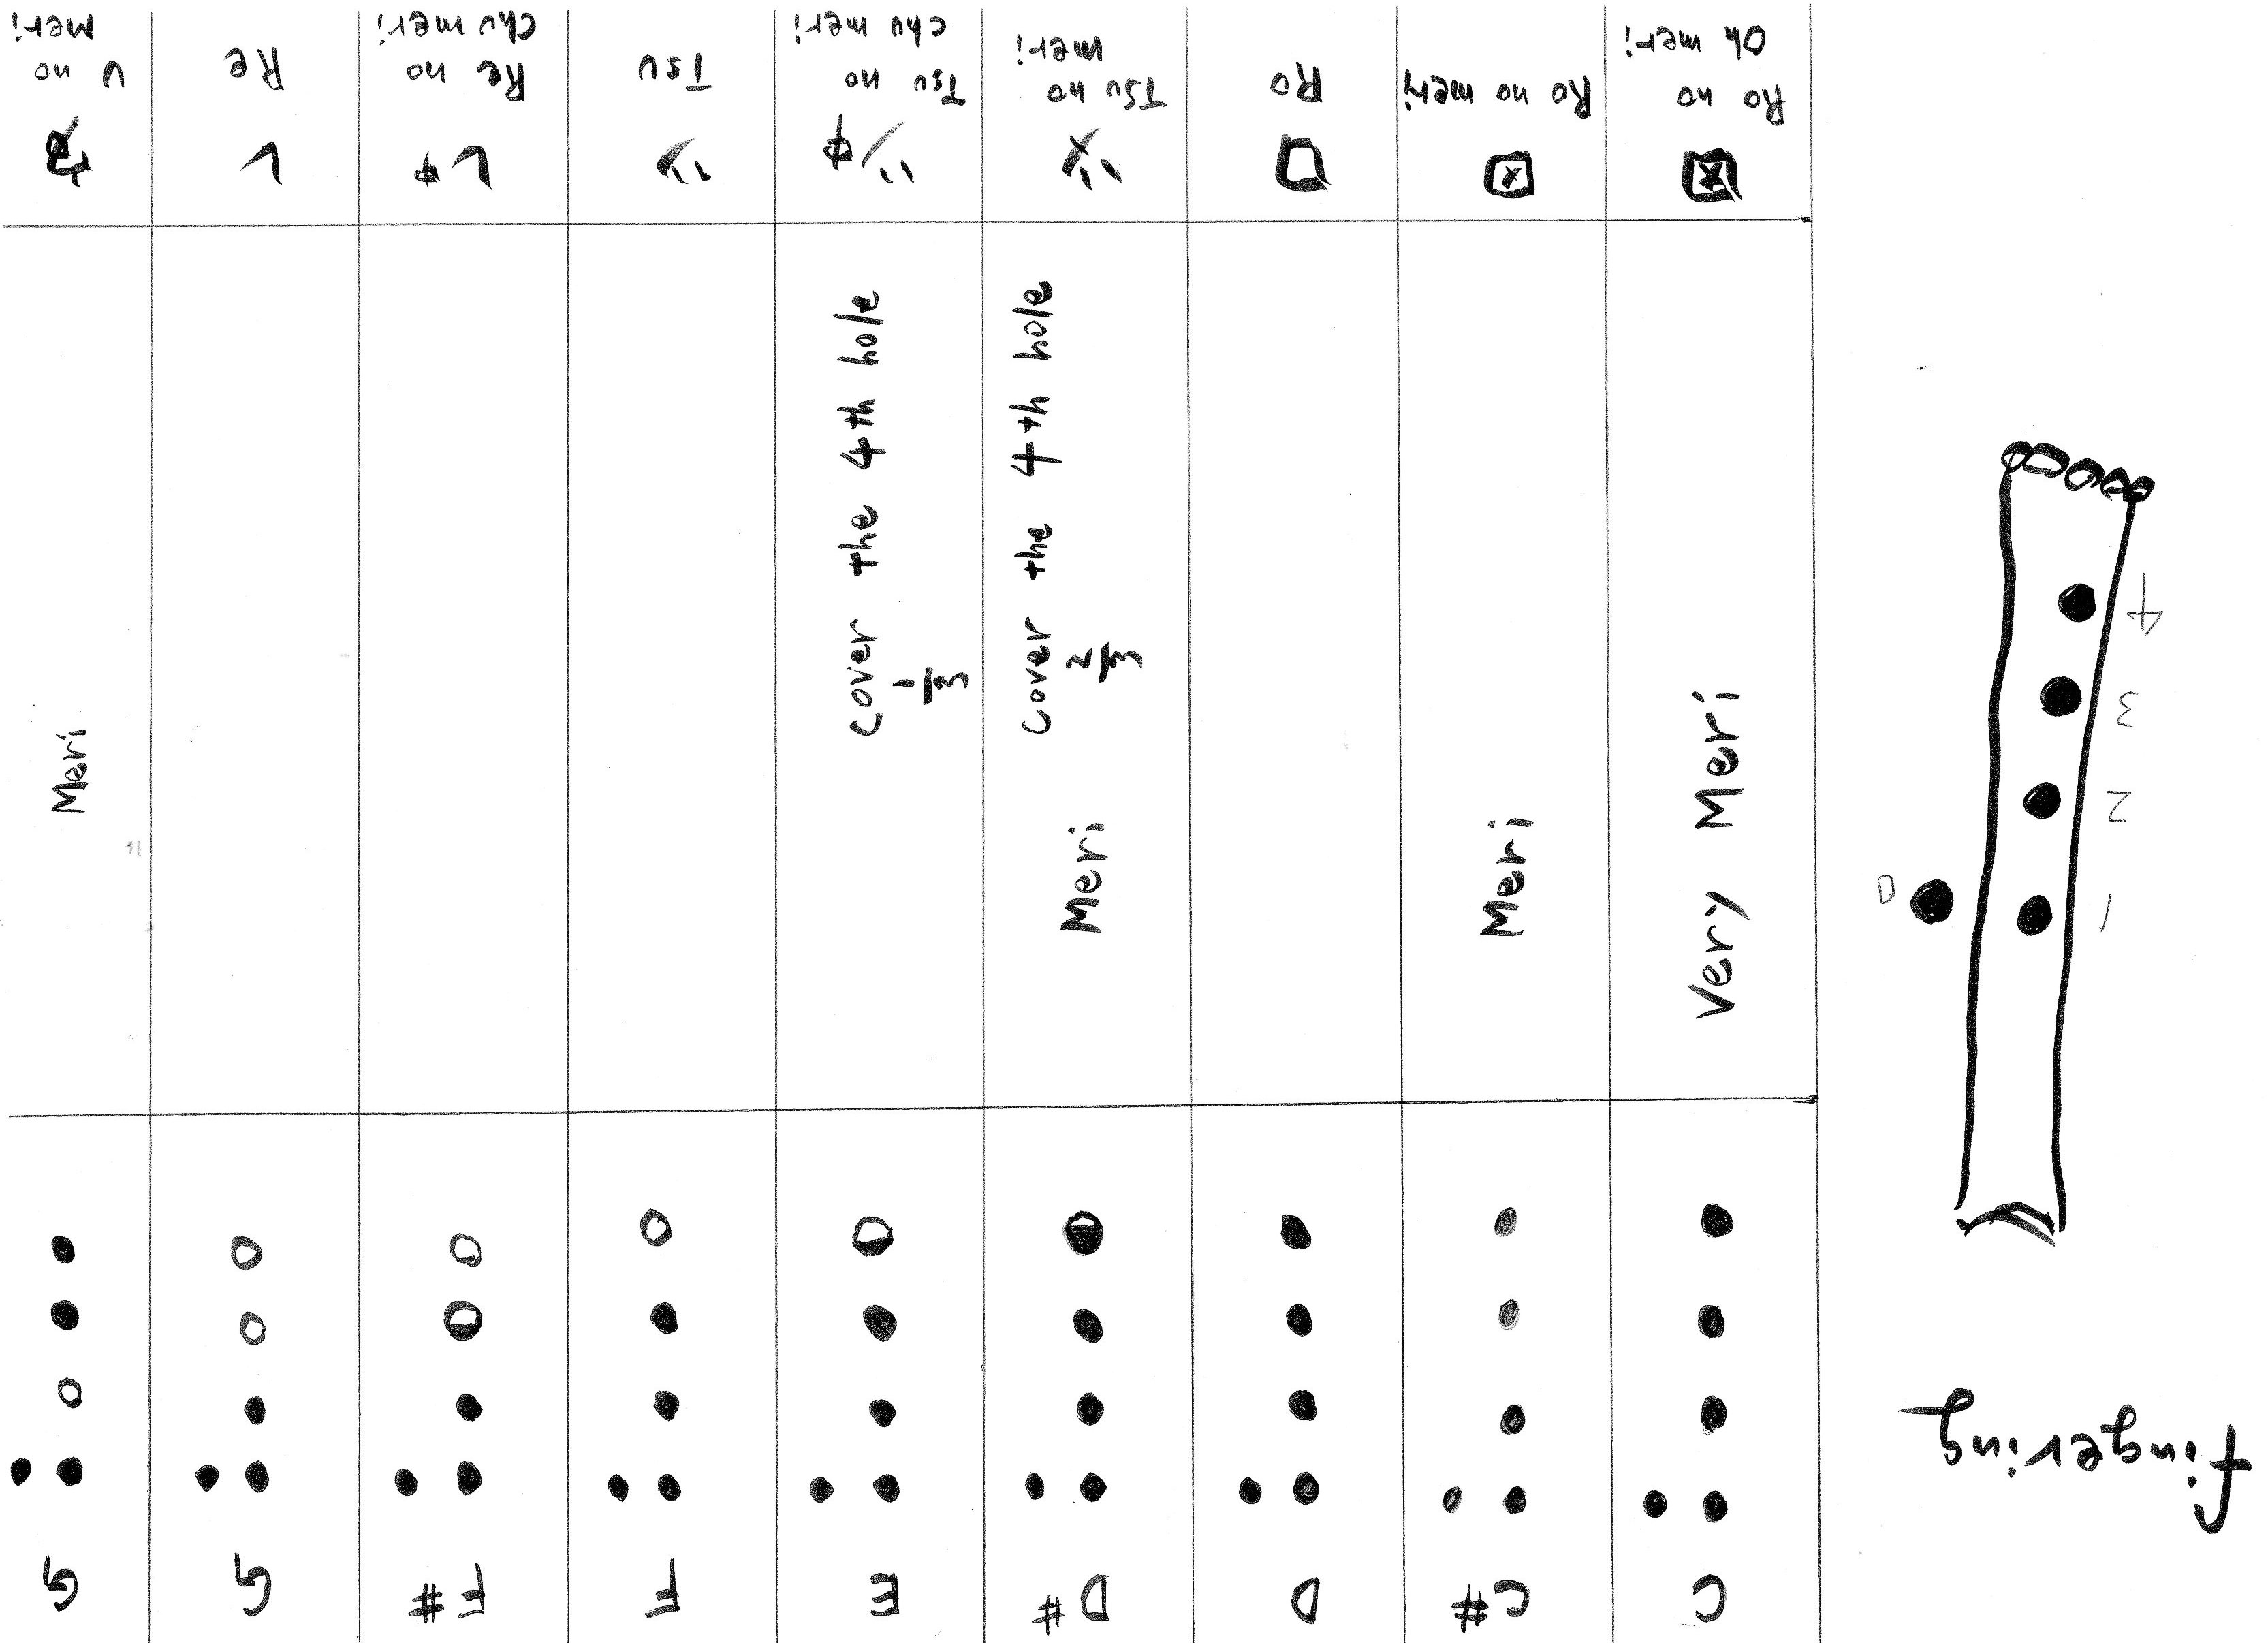
\includegraphics[angle=0,width=1.0\textwidth]{尺八の運指表1}
	\caption{Shakuhachi fingerings Part 1}
	\label{fig:shakuhachi_fingerings_1}
\end{figure}

\begin{figure}[H]
	\centering
	% 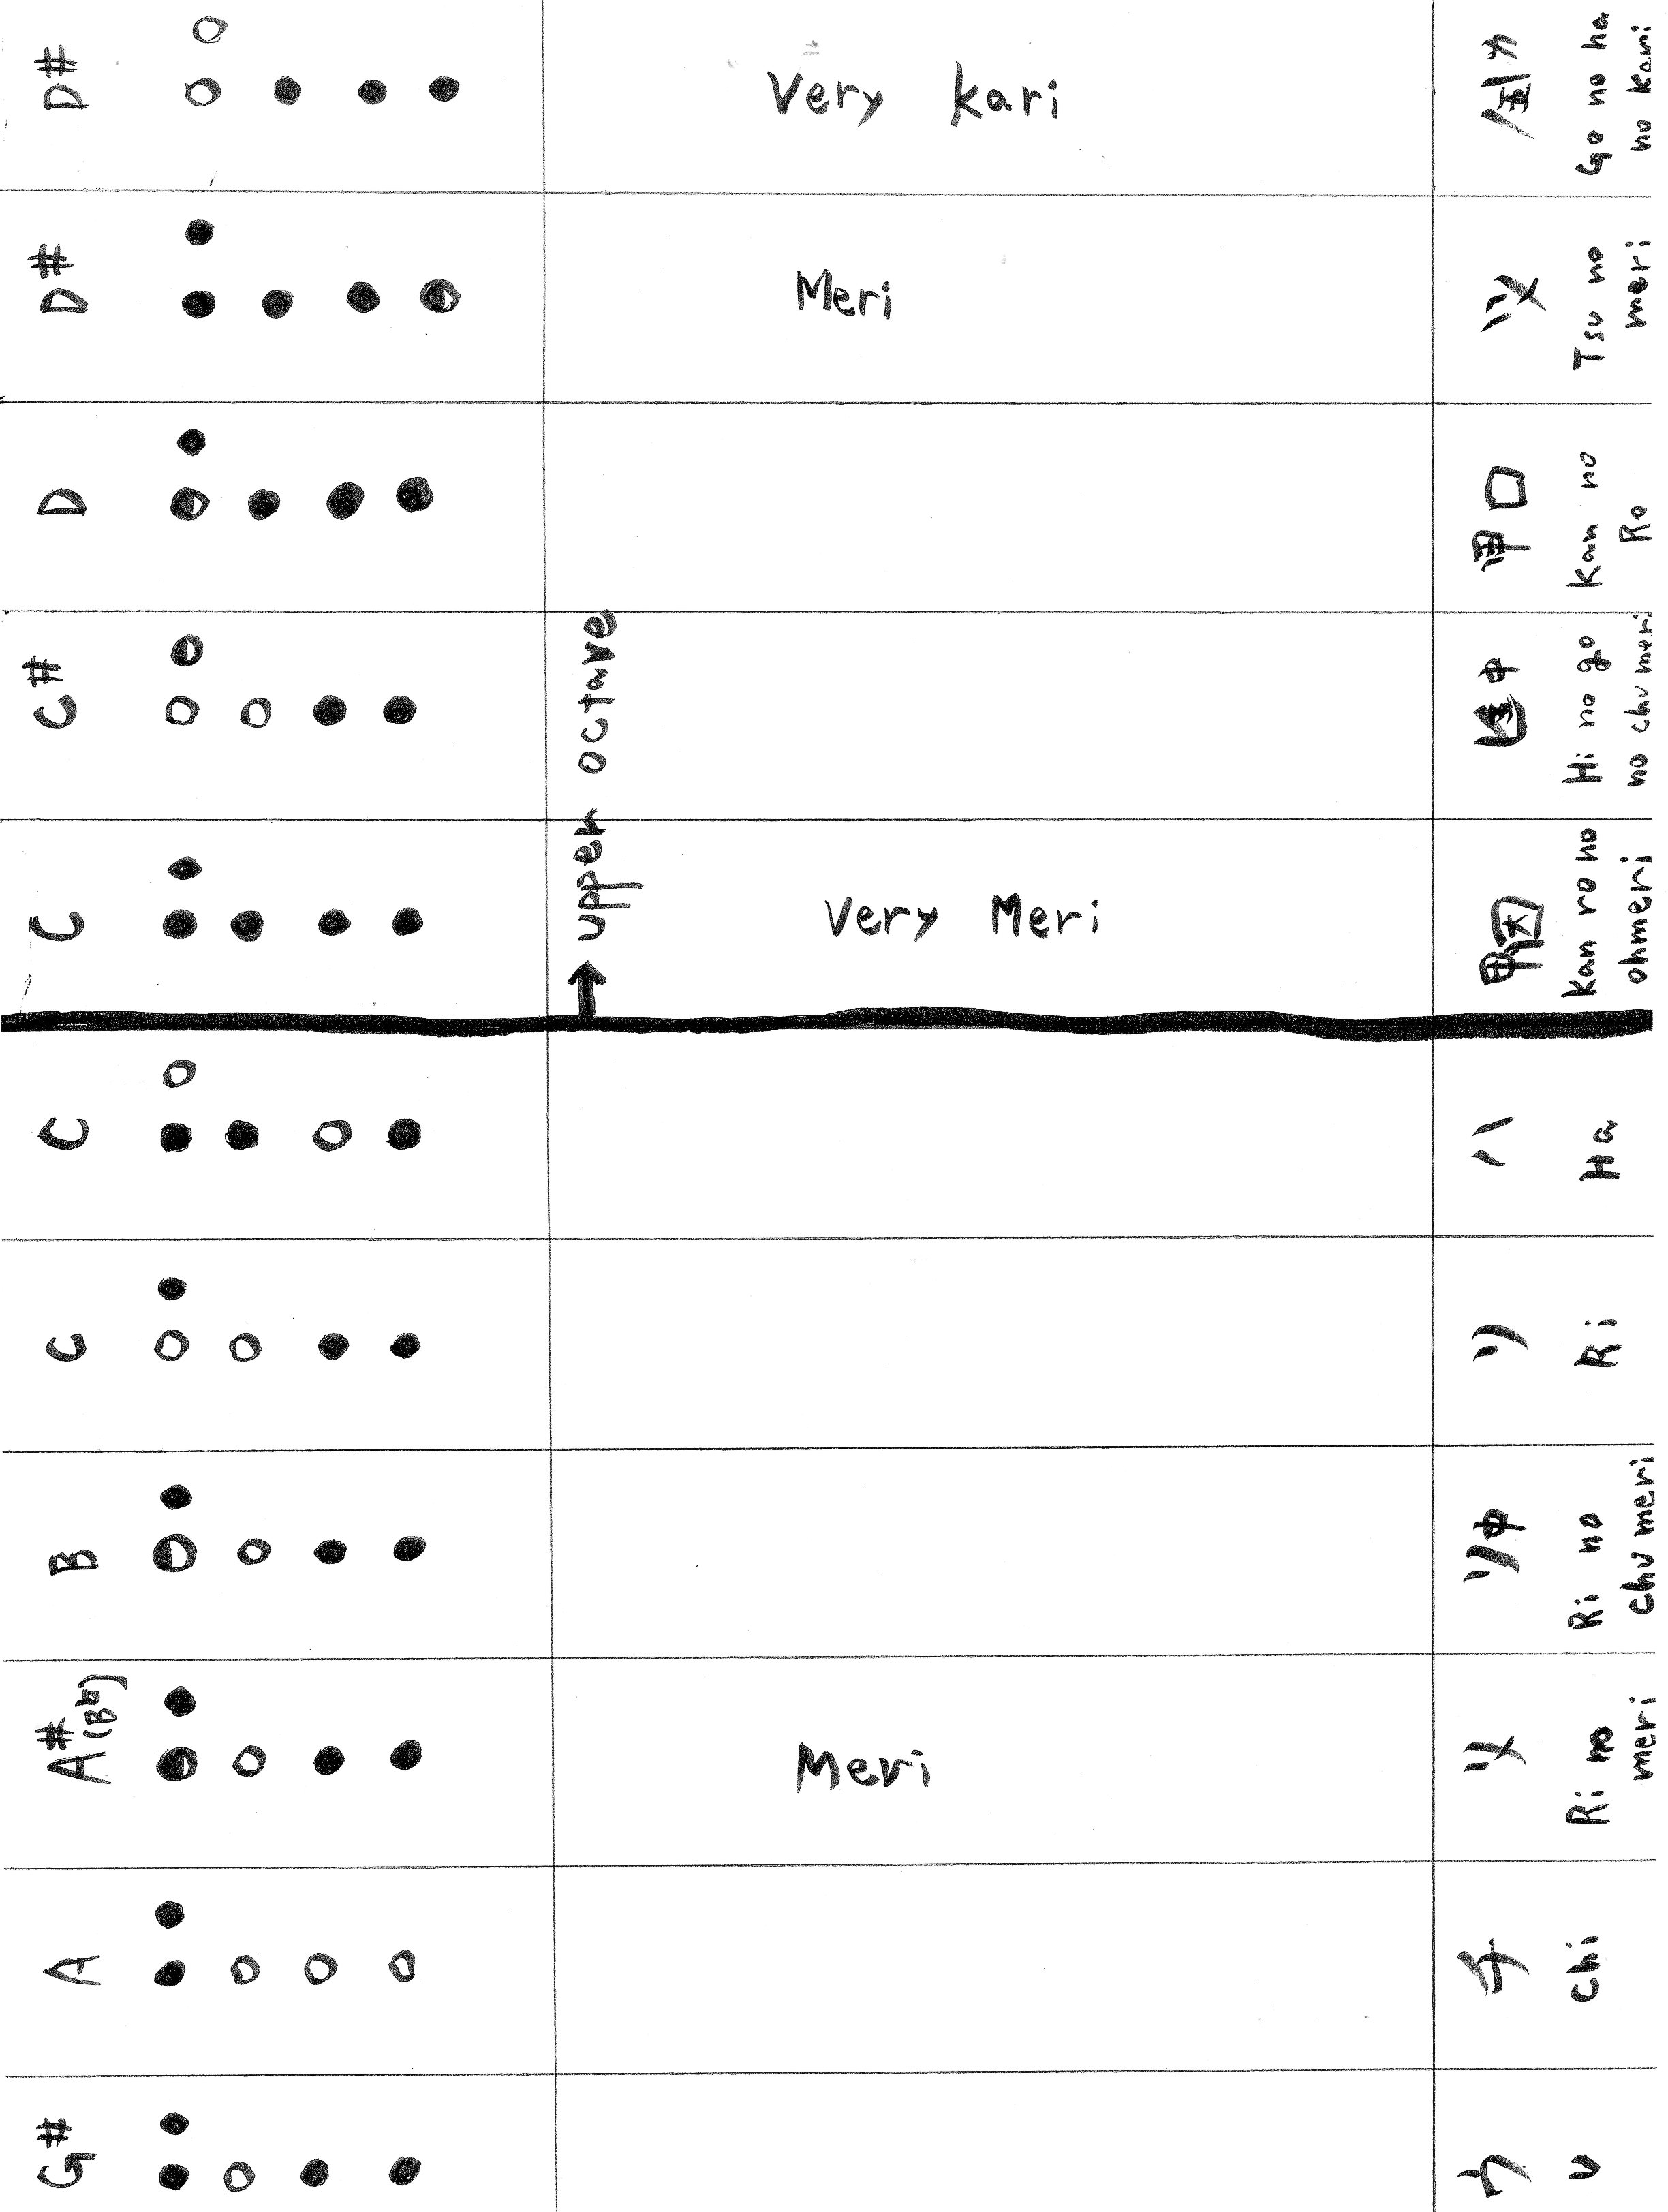
\includegraphics[angle=0,width=1.0\textwidth]{尺八の運指表2}
	\caption{Shakuhachi fingerings Part 2}
	\label{fig:shakuhachi_fingerings_2}
\end{figure}

\begin{figure}[H]
	\centering
	% 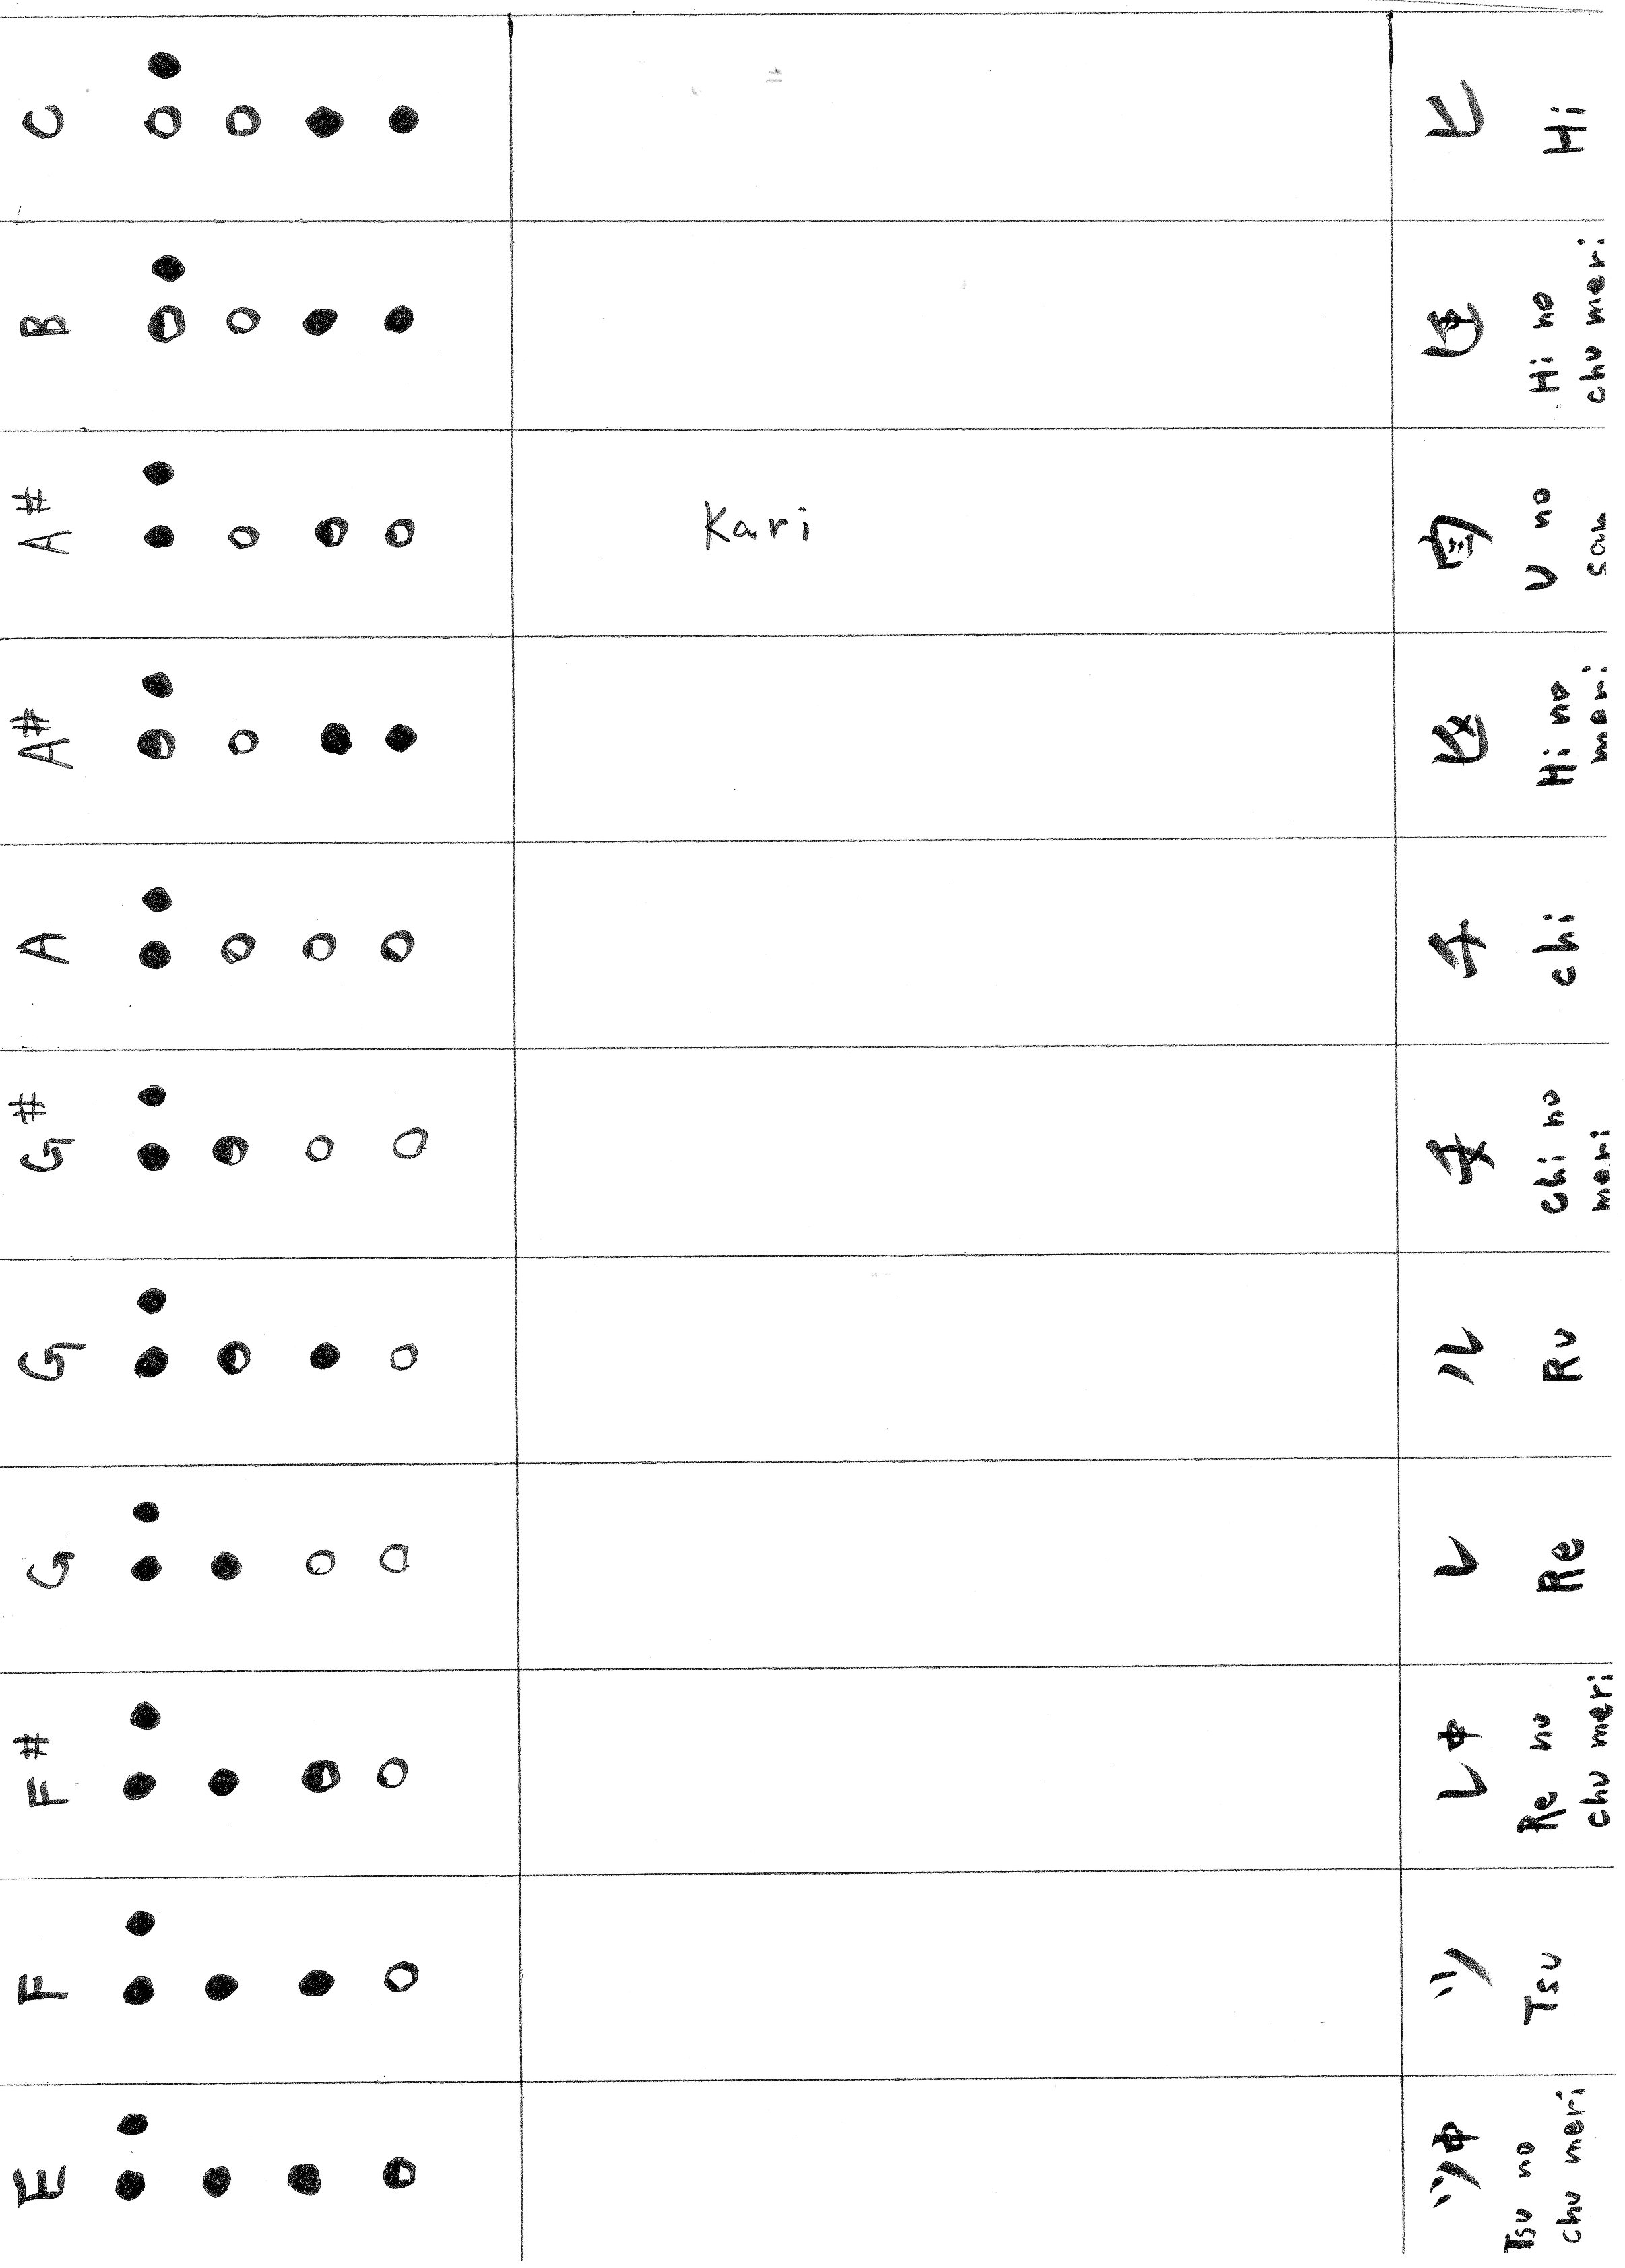
\includegraphics[angle=0,width=1.0\textwidth]{尺八の運指表3}
	\caption{Shakuhachi fingerings Part 3}
	\label{fig:shakuhachi_fingerings_3}
\end{figure}

\begin{figure}[H]
	\centering
	% 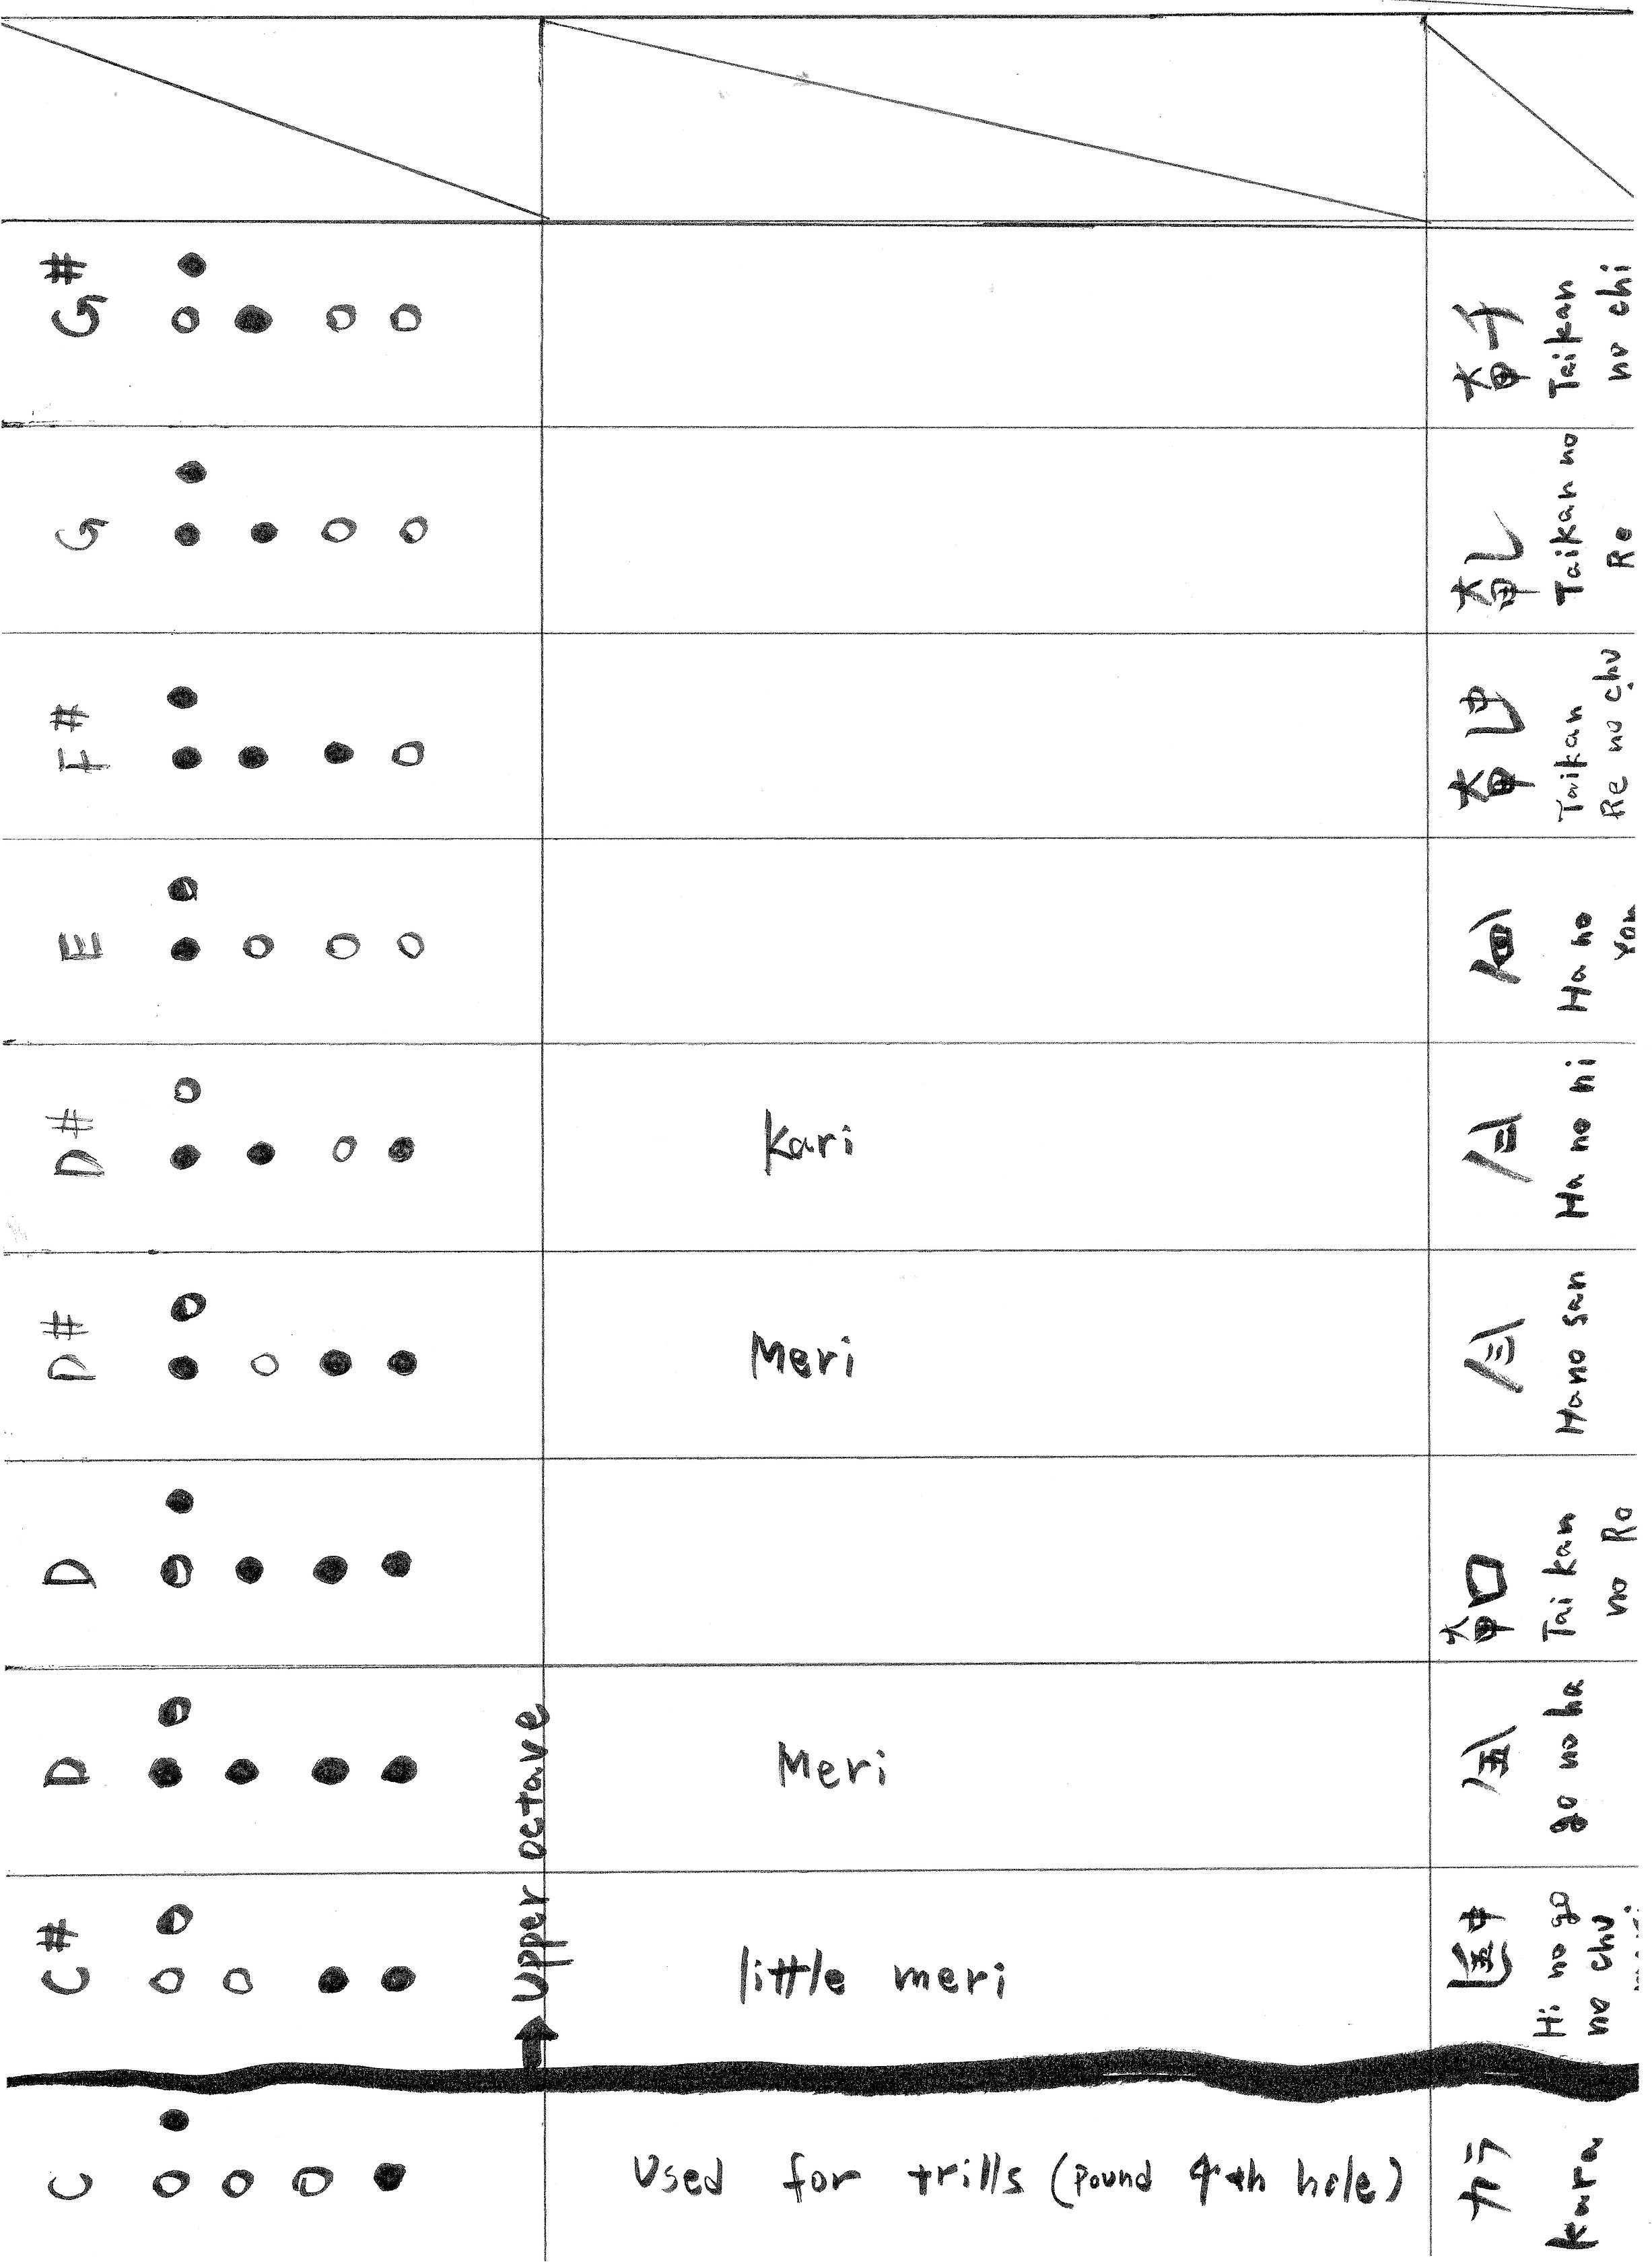
\includegraphics[angle=0,width=1.0\textwidth]{尺八の運指表4}
	\caption{Shakuhachi fingerings Part 4}
	\label{fig:shakuhachi_fingerings_4}
\end{figure}
